\documentclass[english]{article}

%% Packages pull in extra commands:
%% http://en.wikibooks.org/wiki/LaTeX/Packages
\usepackage[latin9]{inputenc}
\usepackage[letterpaper]{geometry}
\geometry{verbose,tmargin=1in,bmargin=1in,lmargin=1in,rmargin=1in}
\usepackage{amsmath}
\usepackage{amssymb}
\usepackage{graphicx}
\usepackage{float}
\usepackage{array}
\usepackage{tikz}
\usepackage{latexsym}
\usepackage{xspace}

% New commands serve as shorthand for frequently used command combinations.
\newcommand{\ind}[1]{\mathbf{1}\left(#1\right)}
\newcommand{\bx}{\mathbf{x}}
\newcommand{\E}{\mathbf{E}}
\newcommand{\bw}{\mathbf{w}}
\renewcommand{\Pr}{\mathbf{Pr}\xspace}
\newcommand{\Bern}{\textsf{Bernoulli}\xspace}
\newcommand{\XX}{\mathcal{X}}

\title{CIS 520, Machine Learning, Fall 2015: Assignment 3}
\author{Yu-Cheng Lin}

\begin{document}
\maketitle
{\normalsize Collaborator: \\ 
\\ \underline{ Type Collaborator Name Here        }

\section{Linear Regression and LOOCV}

%\newcommand{\bw}{\mathbf{w}}

In the last homework, you learned about using cross validation as a
way to estimate the true error of a learning algorithm.  A solution
that provides an almost unbiased estimate of this true error is
\emph{Leave-One-Out Cross Validation} (LOOCV), but it can take a
really long time to compute the LOOCV error.  In this problem, you
will derive an algorithm for efficiently computing the LOOCV error for
linear regression using the \emph{Hat Matrix}.
\footnote{Unfortunately, such an efficient algorithm may not
be easily found for other learning methods.}

Assume that there are $n$ given training examples,
$(X_1,Y_1),(X_2,Y_2),\dots,(X_n,Y_n)$, where each input data point
$X_i$, has $m$ real-valued features.  The goal of regression is to
learn to predict $Y$ from $X$.  The \emph{linear} regression model
assumes that the output $Y$ is a weighted \emph{linear} combination of
the input features with weights given by $\bw$, plus some Gaussian
noise.

We can write this in matrix form by stacking the data points as the
rows of a matrix $X$ so that $x_{ij}$ is the $j$-th feature of the
$i$-th data point.  Then writing $Y$, $\bw$ and $\epsilon$ as column
vectors, we can express the linear regression model in matrix form as
follows:

\[
Y=X\bw + \epsilon
\]

where:

\[
Y = \left[\begin{array}{c}
Y_1 \\
Y_2 \\
\vdots \\
Y_n
\end{array}\right],
X = \left[\begin{array}{cccc}
x_{11} & x_{12} & \dots & x_{1m} \\
x_{21} & x_{22} & \dots & x_{2m} \\
\vdots & \vdots & \ddots & \vdots \\
x_{n1} & x_{n2} & \dots & x_{nm} \\
\end{array}\right],
\bw = \left[\begin{array}{c}
w_1 \\
w_2 \\
\vdots \\
w_m
\end{array}\right],
\,\,\,\,\,\mbox{and}\,\,
\epsilon = \left[\begin{array}{c}
\epsilon_1 \\
\epsilon_2 \\
\vdots \\
\epsilon_n
\end{array}\right]
\]
Assume that $\epsilon_i$ is normally distributed with variance
$\sigma^2$.  We saw in class that the maximum likelihood estimate of
the model parameters $\bw$ (which also happens to minimize the sum of
squared prediction errors) is given by the \emph{Normal equation}:
\[
\hat{\bw} = (X^TX)^{-1} X^TY
\]

\noindent Define $\hat{Y}$ to be the vector of predictions using
$\hat{\bw}$ if we were to plug in the original training set $X$:
\begin{eqnarray*}
\hat{Y} &=& X\hat{\bw}  \\
    &=& X(X^T X)^{-1} X^T Y \\
    &=& H Y
\end{eqnarray*}
where we define $H=X(X^T X)^{-1} X^T$ ($H$ is often called the
\emph{Hat Matrix}).

\noindent As mentioned above, $\hat{\bw}$, also minimizes the sum of
squared errors:
\[
\mbox{SSE} = \sum_{i=1}^{n} (Y_i-\hat{Y}_i)^2
\]
Now recall that the Leave-One-Out Cross Validation score is defined to
be:
\[
\mbox{LOOCV} = \sum_{i=1}^n (Y_i - \hat{Y}_i^{(-i)})^2
\]
where $\hat{Y}^{(-i)}$ is the estimator of $Y$ after removing the
$i$-th observation (i.e., it minimizes $\sum_{j\neq i} (Y_j -
\hat{Y}_j^{(-i)})^2$). 

\begin{enumerate}

\item To begin with, we should consider when it is possible to compute $\hat{\bw}$ in this framework.
	\begin{enumerate}
	\item Suppose $m > n$. Is $\hat{\bw}$ well-defined? Why or why not?\\
	\emph{Hint:} Recall that the rank of a matrix is equal to the number of linearly independent rows, which is also equal to the number of linearly independent columns. Use the fact that for two matrices $A$ and $B$ which can be multiplied to form the product $AB$, it must be the case that $\text{rank}(AB) \le \min \left( \text{rank}(A), \text{rank}(B) \right)$. Furthermore, recall that a square matrix is invertible if and only if it is full-rank.\\
	\\
	
	{\bf Ans: }If $m>n$, $\hat{\bw}$ will not be well defined. This is because that if $m>n$, $X^TX^{-1}$ will have rank $n$ at most while it's a $m \times m$ matrix, and such matrix is not invertible because it's not full rank. \\
	
	\item Suppose $m \le n$. Give a condition on $X$ which guarantees that $\hat{\bw}$ will \textbf{not} be well-defined and explain why not. (Don't assume $X$ is a square matrix.)\\
	\\
	{\bf Ans: } If k columns in $X$ are redundant, $\hat{\bw}$ might not be well defined because $X^TX$ will have rank $n-k$. If $n-k < m$, $X^TX^{-1}$ will not be invertible. \\
	
	\end{enumerate}
For the rest of question 1, assume $\hat{\bw}$ is well-defined.

\item  What is the complexity of computing the LOOCV score
  naively? (The naive algorithm is to loop through each point,
  performing a regression on the $n-1$ remaining points at each
  iteration.)\\
  \\
  {\bf Ans: } Computing LOOCV naively will require $O(n)$ complexity in the outer loop and $O(m^3)$ in the inner loop since I will end up inverting a m by m matrix. Overall, the naive approach should yield a computation complexity of $O(nm^3)$
  \\

  \emph{Hint}: The complexity of matrix inversion for a $k\times k$
  matrix is $O(k^3)$.  (There are faster algorithms out there but for
  simplicity we'll assume that we are using the naive $O(k^3)$
  algorithm.)


\item  Write $\hat{Y}_i$ in terms of the elements of $H$ and
  $Y$.  You may find it useful to use shorthand such as $H_{ab}$ to
  denote the entry in row $a$, column $b$ of $H$.
  \\
  \\{\bf Ans: }
  \[\hat{Y}_i = \sum_{J=1}^{m}H_{ij}Y_j \]


\item Show that $\hat{Y}^{(-i)}$ is also the estimator
  which minimizes SSE for $Z$ where
  \[
  Z_j = \left\{\begin{array}{cc}
  Y_j, & j\neq i \\
  \hat{Y}_i^{(-i)}, & j=i \\
  \end{array}\right.
  \]

  \emph{Hint}: Try to start by writing an expression for the SSE of
  $Z$; it should look very similar to the definition of SSE for $Y$
  that was given in the introduction section of this question.  Then,
  manipulate terms until you can argue that substituting
  $\hat{Y}^{(-i)}$ for $\hat{Z}$ would minimize this expression.
  \\
    \\
    {\bf Ans: }
    We first write the SSE for Z
    \[SSE_Z =  \sum^n_{j = 1}(Z-\hat{Y}^{(-i)})^2\]
    Now substitute Z
  \[
  SSE_Z = \left\{\begin{array}{cc}
  \sum_{j=1}^n (Y_j - \delta_{ij}\hat{Y}_i^{(-i)})^2 & j \neq i \\
  (\hat{Y}_i^{(-i)} - \hat{Y}_i^{(-i)})^2 & j = i \\
  \end{array}\right.
  \]    
    As we can see, when $j = i$, the SSE is zero, otherwise it takes the same form as the SSE of Y. In conclusion, $\hat{Y}^{(-i)}$ for $\hat{Z}$ would minimize Z.


\item   Write $\hat{Y}_i^{(-i)}$ in terms of $H$ and $Z$. By
definition, $\hat{Y}_i^{(-i)} = Z_i$, but give an answer that includes both
$H$ and $Z$.
\\
 {\bf Ans: }
\[
\hat{Y}_i^{(-i)} = \sum_{j=1}^m H{ij}Z_j
\]
\\
\item  \label{it:diag}
Show that $\hat{Y}_i - \hat{Y}_i^{(-i)} = H_{ii}Y_i - H_{ii}\hat{Y}_i^{(-i)}$,
where $H_{ii}$ denotes the $i$-th element along the diagonal of $H$.\\
 \emph{Hint}: Use the results from  part 2 and 4. Substitute $Z_i$ with $Y_i$ and $\hat{Y}_i^{-i}$ by using its definition in part 3.

 {\bf Ans: }
\begin{align*}
	\hat{Y}_i - \hat{Y}_i^{(-i)} =&\; \sum_{J=1}^{m}H_{ij}Y_j - \sum_{j=1}^m 		H{ij}Z_j\\
	=&\; \sum_{J=1}^{m}H_{ij}Y_j - (\sum_{j=1}^m H_{ij}Y_j - H_{ii}Y_i + H_{ii}\hat{Y}_i^{(-i)}\\
	=&\; H_{ii}Y_i - H_{ii}\hat{Y}_i^{(-i)}
\end{align*}



\item 
Show that
\[
LOOCV = \sum_{i=1}^{n}  \left(\frac{Y_i - \hat{Y}_i}{1-H_{ii}}\right)^2
\]
What is the algorithmic complexity of computing the LOOCV score using
this formula?

Note: We see from this formula that the diagonal elements of $H$ somehow
indicate the impact that each particular observation has on the result
of the regression.\\
\\
use the result from (6) and solve for $\hat{Y}_i^{(-i)}$:
\begin{align*}
\hat{Y}_i - \hat{Y}_i^{(-i)} =&\; H_{ii}Y_i - H_{ii}\hat{Y}_i^{(-i)}\\
\hat{Y}_i - H{ii}Y_i =&\; (1-H_{ii})\hat{Y}_i^{(-i)}\\
\hat{Y}_i^{(-i)}=&\; \frac{\hat{Y}_i-H_{ii}Y_i}{1-H_{ii}}
\end{align*}
plug this $\hat{Y}_i^{(-i)}$ in the LOOCV formula and do some algebra:
\begin{align*}
LOOCV =&\; \sum_{i=1}^{n}  \left(Y_i - \hat{Y}_i^{(-i)}\right)^2\\
=&\; \sum_{i=1}^{n}  \left(Y_i - \frac{\hat{Y}_i-H_{ii}Y_i}{1-H_{ii}}\right)^2\\
=&\; \sum_{i=1}^{n}  \left(\frac{Y_i - \hat{Y}_i}{1-H_{ii}}\right)^2
\end{align*}
\end{enumerate}

\section{Logistic regression and Naive Bayes }

A common debate in machine learning has been over generative versus
discriminative models for classification.  In this question we will
explore this issue by considering Naive Bayes and logistic regression.

\begin{enumerate}
\item  For input $X$ and output $Y$, which of the
  following is the {\bf objective function} optimized by (i) Naive
  Bayes, and (ii) logistic regression?
  \begin{enumerate}
  \item $\Pr(Y) / \Pr(X)$
  \item $\Pr(X) / \Pr(Y)$
  \item $\Pr(Y \mid X)$  Logistic regression optimizes this function, which is discriminative
  \item $\Pr(Y)$
  \item $\Pr(X)$
  \item $\Pr(Y) \Pr(X)$
  \item $\Pr(X, Y)$  Naive Bayes optimizes this function, which is generative
  \item None of the above (provide the correct formula in this case)
  \end{enumerate}


\item Recall from the suggested reading that ``the
  discriminative analog of Naive Bayes is logistic regression.'' This
  means that the parametric form of $P(Y \mid X)$ used by logistic
  regression is implied by the assumptions of a Naive Bayes
  classifier, for some specific class-conditional densities. In class
  you will see how to prove this for a Gaussian Naive Bayes classifier
  for continuous input values. Can you prove the same for binary
  inputs? Assume $X_i$ and $Y$ are both binary. Assume that $X_i \mid
  Y=j$ is $\Bern (\theta_{ij})$, where $j \in \{0,1\}$, and $Y$ is
  $\Bern(\pi)$.
\emph{Hint:} Start by using Bayes Rule and the assumptions of Naive Bayes to express the objective function for logistic regression in terms of the given quantities $\theta_{ij}$ and $\pi$.
\\
\\{\bf ANS: }
Let's start with the probabilities
\begin{align*}
P(X_i, Y = j) =&\; \theta_{ij}\\
P(Y = 1) =&\; \pi\\
P(Y = 0) =&\; 1 - \pi
\end{align*}
The goal of logistic regression is to maximize the following target function
\begin{align*}
P(Y = 1 | X_{1, 2, 3 ..., n}) =&\; \frac{P(X_{1, 2, 3 ..., n} | Y = 1)P(Y=1)}{P(X_{1, 2, 3 ..., n})}\\
 \text{marginalize to obtain} \\
=&\; \frac{P(X_{1, 2, 3 ..., n} | Y = 1)P(Y=1)}{P(X_{1, 2, 3 ..., n}|Y=1)(Y=1)+P(X_{1, 2, 3 ..., n}|Y=0)(Y=0)}\\
 =&\; \frac{1}{1+\frac{P(X_{1, 2, 3 ..., n}|Y=0)P(Y=0)}{P(X_{1, 2, 3 ..., n}|Y=1)P(Y=1)}}\\
 =&\; \frac{1}{1 + \exp(\ln(\frac{P(Y=0)}{P(Y=1)}) + \ln(\frac{P(X_{1, 2, 3 ..., n}|Y=0)}{P(X_{1, 2, 3 ..., n}|Y=1}))}\\
 =&\; \frac{1}{1 + \exp(\ln(\frac{1-\pi}{\pi}) + \ln(\frac{\prod_{i = 1}^n \theta_{i0}}{\prod_{i = 1}^n \theta_{i1}}))}\\
 =&\; \frac{1}{1 + \exp(\ln(\frac{1-\pi}{\pi}) + \sum_{i=1}^n\ln(\frac{\theta_{i0}}{\theta_{i1}}))}
\end{align*}

from here, we can plug in the definition of Bernoulli distribution for $\theta_{ij}$

\[
\theta_{ij} = \theta_{ij}^{X_i}(1-\theta_{ij})^{1-X_i}
\]
We obtain
\begin{align*}
\frac{1}{1 + \exp(\ln(\frac{1-\pi}{\pi}) + \sum_{i=1}^n\ln(\frac{\theta_{i0}}{\theta_{i1}}))} 
=&\; \frac{1}{1 + \exp(\ln(\frac{1-\pi}{\pi}) + \sum_{i=1}^n\ln(\frac{\theta_{i0}^{X_i}(1-\theta_{i0})^{1-X_i}}{\theta_{i1}^{X_i}(1-\theta_{i1})^{1-X_i}}))}
\end{align*}

the terms inside the natural log can be simplified as
\begin{align*}
\ln(\frac{\theta_{i0}^{X_i}(1-\theta_{i0})^{1-X_i}}{\theta_{i1}^{X_i}(1-\theta_{i1})^{1-X_i}}) 
=&\;
\ln((\frac{\theta_{i0}}{\theta_{i1}})^{X_i}(\frac{1-\theta_{i0}}{1-\theta_{i1}})^{1 - Xi})\\
=&\;
\frac{\frac{\theta_{i0}}{\theta_{i1}}}{\ln(\frac{\theta_{i0}}{\theta_{i1}})}X_i + \frac{\frac{1-\theta_{i0}}{1-\theta_{i1}}}{\ln(\frac{1-\theta_{i0}}{1-\theta_{i1}})}(1-X_i)
\end{align*}
Which is in form
\[
w_iX_i + K_i
\]

Ultimately, plugging this term back in the original equation, we will get the objective function of logistic regression
\[
\frac{1}{1 + \exp(w_0 + \sum_{i=1}^n w_iX_i)}
\]

\end{enumerate}

\section{Double-counting the evidence}

\begin{enumerate}
\item Consider the two class problem where class label $y
  \in \{T, F\}$ and each training example $X$ has 2 binary attributes
  $X_1, X_2 \in \{T, F\}$. How many parameters will you \emph{need} to
  know/evaluate if you are to classify an example using the Naive
  Bayes classifier?  Keep in mind that since the probability of all
  possible events has to sum to 1, knowing the probabilities of all
  except one event implies knowledge of the final event's probability
  already.  (Don't include such final events in your count.)
  \\
  \\{\bf ANS: }
  We need four parameters to use this Naive Bayes classifier.
  \begin{align*}
  P(X_1 = T | Y = T)\\
  P(X_2 = T | Y = T)\\
  P(X_1 = T | Y = F)\\
  P(X_2 = T | Y = F)\\
  \end{align*}
  

\item Let the class prior be $\Pr(Y=T)=0.5$ and also let
  $\Pr(X_1=T \mid Y=T) = 0.8$, $\Pr(X_1=F \mid Y=F) = 0.7$, $\Pr(X_2=T
  \mid Y=T) = 0.5$, and $\Pr(X_2=F \mid Y=F) = 0.9$. (\emph{Note:} Questions 3.2 - 3.4 all use these probabilities.) So, attribute
  $X_1$ provides slightly stronger evidence about the class label than
  $X_2$.  Assume $X_1$ and $X_2$ are truly independent given
  $Y$. Write down the Naive Bayes {\bf decision rule} given $X_1=x_1$
  and $X_2=x_2$.  Write your answer as a table listing the value of
  the decision, call it $f(X_1, X_2)$, for each of the 4 settings for
  $X_1, X_2$.
\\
\\{\bf ANS:} 
Let's first write out the decision rule of Naive Bayes
\[
\frac{P(Y=T)\prod_{i=1}^n P(X_i|Y = T)}{P(Y=F)\prod_{i=1}^n P(X_i|Y=F)} \geq 1
\]
If the inequality above holds true, Naive Bayes will return Y = T\\
Following is a table of the 4 possible scenarios:\\
\\
\begin{center}
\begin{tabular}{| >{$}l<{$} | >{$}l<{$} | >{$}l<{$}|}
\hline
X_2/X_1 & X_1 = T                                             & X_1 = F\\ \hline
X_2 = T & \frac{(0.5)(0.8)(0.5)}{(0.5)(0.3)(0.1)} = 13.3 > 1  & \frac{(0.5)(0.8)(0.5)}{(0.5)(0.3)(0.9)} = 1.48 > 1\\
\hline
X_2 = F & \frac{(0.5)(0.2)(0.5)}{(0.5)(0.7)(0.1)} = 1.42 > 1  & \frac{(0.5)(0.2)(0.5)}{(0.5)(0.7)(0.9)} = 0.158 <1\\ \hline
\end{tabular}
\end{center}
such results in the following truth table:
\\
\begin{center}
\begin{tabular}{| >{$}l<{$} | >{$}l<{$} | >{$}l<{$}|}
\hline
X_2/X_1 & X_1 = T                                             & X_1 = F\\ \hline
X_2 = T & T  & T\\
\hline
X_2 = F & T  & F\\ \hline
\end{tabular}
\end{center}
  
\item For the Naive Bayes decision function $f(X_1, X_2)$,
  the error rate is:
  \begin{equation*}
    \sum_{X_1,X_2,Y} \ind{Y \ne f(X_1,X_2)}P(X_1, X_2, Y).
  \end{equation*}
  For this question, we will assume that the true data distribution is
  exactly the same as the Naive Bayes distribution, so we can write
  $P(X_1, X_2, Y)$ as $P(Y)P(X_1 \mid Y)P(X_2 \mid Y)$.

  \begin{enumerate}
    \item  Show that if Naive Bayes uses both attributes,
      $X_1$ and $X_2$, the error rate is $0.235$.
  \\{\bf ANS:}
  There are four scenarios which gives me an error:
  \begin{align*}
  P(Y = F, X_1 = T, X_2 = T) =&\; P(Y = F)P(X_1 = T \mid Y = F)P(X_2 = T \mid Y = F) = (0.3)(0.1)(0.5) = 0.015\\
  P(Y = F, X_1 = F, X_2 = T) =&\; P(Y = F)P(X_1 = F \mid Y = F)P(X_2 = T \mid Y = F) = (0.7)(0.1)(0.5) = 0.035\\
  P(Y = F, X_1 = T, X_2 = F) =&\; P(Y = F)P(X_1 = T \mid Y = F)P(X_2 = F \mid Y = F) = (0.3)(0.9)(0.5) = 0.135\\
  P(Y = T, X_1 = F, X_2 = F) =&\; P(Y = T)P(X_1 = F \mid Y = T)P(X_2 = F \mid Y = T) = (0.7)(0.5)(0.5) = 0.05
  \end{align*}
  Sum all the probability up, we obtain:
  \[
  0.015 + 0.035 + 0.135 + 0.05 = 0.235
  \]
    \item  What is the error rate using only $X_1$?
    \\
    \\{\bf ANS:}
    Since we can just read the decision rule off of one variable, I will not compute the decision rule for part b and c.\\
    There are two scenarios which gives me an error:
    \begin{align*}
    P(Y = F, X_1 = T) =&;\ (0.3)(0.5) = 0.15\\
    P(Y = T, X_1 = F) =&;\ (0.2)(0.5) = 0.1\\   
    \end{align*}
    The error rate sums up to 0.25.

    \item  What is the error rate using only $X_2$?
    \\
    \\{\bf ANS:}
    \begin{align*}
    P(Y = F, X_2 = T) =&;\ (0.1)(0.5) = 0.05\\
    P(Y = T, X_2 = F) =&;\ (0.5)(0.5) = 0.25\\   
    \end{align*}
    The error rate sums up to 0.3.

    \item  Give a conceptual explanation for why the error rate is (choose one) lower/higher using $X_1$ and $X_2$ together as opposed to using only a single attribute.
    \\
    \\{\bf ANS:}
    In this case, the error rate is lower when both $X_1$ and $X_2$ are used.  Given that my assumptions of Naive Bayes are correct, obtaining each feature gives some additional information gain to help me predict the outcome better. 
            
  \end{enumerate}

\item Now, suppose that we create a new attribute $X_3$,
  which is an exact copy of $X_2$. So, for every training example,
  attributes $X_2$ and $X_3$ have the same value, $X_2 = X_3$.

  \begin{enumerate}
  \item Are $X_2$ and $X_3$ conditionally independent given
    $Y$? 
    \\
    \\{\bf ANS:}
    They are not conditionally independent given Y because
    \[
    P(X_3 = T | Y, X_2 = T) = 1
    \]
    If they are truely conditionally independent,
    \[
    P(X_3 = T | Y, X_2 = T) = 0.3 = P(X_3 = T | Y)
    \]
    which is untrue

  \item What is the error rate of Naive Bayes now, using
    $X_1$, $X_2$, and $X_3$? The predicted $Y$ should be computed using the (possibly incorrect) assumption of conditional independence, and the error rate should be computed using the true probabilities.

Here I will save work and space by not considering $X_2 \neq X_3$ since such scenario is impossible

\begin{center}
\begin{tabular}{| >{$}l<{$} | >{$}l<{$} | >{$}l<{$}|}
\hline
X_2/X_1 & X_1 = T                                             & X_1 = F\\ \hline
X_2 = X_3 = T & \frac{(0.5)(0.8)(0.5)(0.5)}{(0.5)(0.3)(0.1)(0.1)} = 66 > 1  & \frac{(0.5)(0.8)(0.5)(0.5)}{(0.5)(0.3)(0.9)(0.9)} = 0.822 < 1\\
\hline
X_2 = X_3 = F & \frac{(0.5)(0.2)(0.5)(0.5)}{(0.5)(0.7)(0.1)(0.1)} = 7.1 > 1  & \frac{(0.5)(0.2)(0.5)(0.5)}{(0.5)(0.7)(0.9)(0.9)} = 0.087 <1\\ \hline
\end{tabular}
\end{center}
such results in the following truth table:
\\
\begin{center}
\begin{tabular}{| >{$}l<{$} | >{$}l<{$} | >{$}l<{$}|}
\hline
X_2/X_1 & X_1 = T                                             & X_1 = F\\ \hline
X_2 = X_3 = T & T  & F\\
\hline
X_2 = X_3 = F & T  & F\\ \hline
\end{tabular}
\end{center}
Now, let's calculate the error rate, note that since $X_3 = X_2$
\[
 	 P(X_3| Y, X_2) = 1
\]
\[
	P(X_3, X_2 | Y) = P(X_2 | Y)
\]

Again, four scenarios will give me error

  \begin{align*}
  P(Y = F, X_1 = T, X_2 = T, X_3 = T) =&\; P(Y = F)P(X_1 = T \mid Y = F)P(X_2 = T \mid Y = F) \\
=&\; (0.3)(0.1)(0.5)(1) = 0.015\\
  P(Y = F, X_1 = F, X_2 = T, X_3 = T) =&\; P(Y = F)P(X_1 = F \mid Y = F)P(X_2 = T \mid Y = F) \\
=&\; (0.7)(0.1)(0.5)(1) = 0.035\\
  P(Y = T, X_1 = T, X_2 = F, X_3 = F) =&\; P(Y = T)P(X_1 = T \mid Y = T)P(X_2 = F \mid Y = T) \\
=&\; (0.8)(0.5)(0.5)(1) = 0.2\\
  P(Y = T, X_1 = F, X_2 = F, X_3 = F) =&\; P(Y = T)P(X_1 = F \mid Y = T)P(X_2 = F \mid Y = T) \\
=&\; (0.7)(0.5)(0.5) = 0.05
  \end{align*}
  The error rate sums up to be 
  \[
  0.015 + 0.2 + 0.035 + 0.05 = 0.3
  \]
    
  \end{enumerate}

\item Why does Naive Bayes perform worse with the addition
  of $X_3$?  (\emph{Hint}: What assumption does Naive Bayes make about
  the inputs?)
  \\
  \\{\bf ANS:}
  When we added $X_3$, the problem does not satisfy the assumption of Naive Bayes anymore. We can see that the decision rule essentially throws out $X_1$ and becomes the same as when we only considered $X_2$. The error rate moves torwards the error rate of only $X_2$ as the result.


\item Does logistic regression suffer from the same
  problem?  Explain why or why not.
  
{\bf ANS:}
  Logistic regression does not suffer from this problem because logistic regression makes no assumption about X.

\item : In spite of the above fact we
  will see that in some examples Naive Bayes doesn't do too
  badly. Consider the above example i.e. your features are $X_1$,
  $X_2$ which are truely independent given $Y$ and a third feature
  $X_3=X_2$.  Suppose you are now given an example with $X_1 = T$ and
  $X_2 = F$.  You are also given the probabilities $\Pr(Y=T \mid
  X_1=T)=p$ and $Pr(Y=T \mid X_2=F)=q$, and $P(Y=T) = 0.5$. (\emph{Note:} You should \textbf{not} use the probabilities from 3.2-3.4 in your solutions to the following.)

  \begin{enumerate}
    \item Prove that the decision rule is $p \ge \frac{(1-q)^2}{q^2 +
      (1-q)^2}$ by applying Bayes rule again.
	\\
  	\\{\bf ANS:}
  	Let's apply Baye's rule to first
  	\begin{align*}
  	P(X_1 | Y = T) = \frac{pP(X_1)}{0.5}\\
  	P(X_1 | Y = F) = \frac{(1-p)P(X_1)}{0.5}\\
  	P(X_2 | Y = T) = \frac{qP(X_2)}{0.5}\\
  	P(X_2 | Y = f) = \frac{(1-q)P(X_2)}{0.5}
  	\end{align*}
  	
  	As we can see, when we take the fraction of one feature given $Y = T$ and $Y = F$, the $P(X)$ and $P(Y)$ cancels out. I can then write the decision rule as follows
  	\[
  	\frac{P(Y=T) \prod_i^n P(Y=T|X_i = T)}{P(Y=F) \prod_i^n P(Y=F|X_i = F)} \geq 1
  	\]
  	gives me $Y=T$//
  	So the product ends up being
  	
  	\begin{align*}
  	\frac{pq^2}{(1-p)(1-q)^2} \geq &\; 1\\
  	pq^2 \geq &\; (1-p)(1-q)^2 \\
  	pq^2 \geq &\; (1-q)^2 - p(1-q)^2 \\
  	pq^2 + p(1-q)^2 \geq &\; (1-q)^2 \\
  	p \geq &\; \frac{(1-q)^2}{q^2 + (1-q)^2}
  	\end{align*}


    \item What is the true decision rule?
\\
\\{\bf ANS:} The true decision rule can be obtained by simply taking out double counting
\[
p \geq \frac{(1-q)}{q + (1-q)} = 1-q
\]

    \item Plot the two decision boundaries (vary $q$ between $0$ and
      $1$) and highlight the region where Naive Bayes makes mistakes.
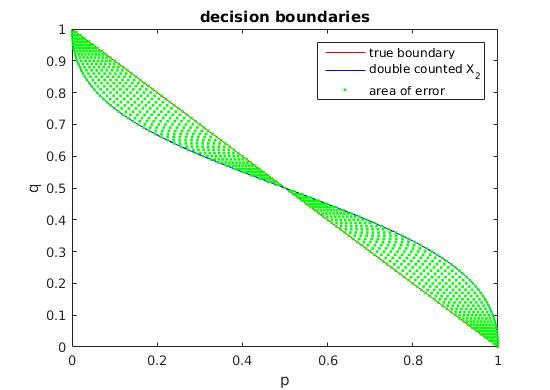
\includegraphics[scale=0.7]{decision_boundary.jpg}
      %% Don't remove the empty line below.  Compilation will fail.
      
  \end{enumerate}
\end{enumerate}

\section{Feature Selection}
We saw in class that one can use a variety of regularization penalties in linear regression.

$$\hat{w} = \arg \min_w  \quad \|Y - Xw\|_2^2 + \lambda \|w\|_p^p$$

Consider the three cases, $p$ = 0, 1, and 2. We want to know what
effect these different penalties have on estimates of $w$.

Let's see this using a simple problem. 

Use the following data (also provided in matlab format).  Assume the
constant term in the regression is zero, and assume $\lambda=1$,
except, of course, for question (1).  You don't need to write code
that solves these problems in their full generality; instead, feel
free to use matlab to do the main calculations, and then just do a
primitive search over parameter space by plugging in a few different
values. Matlab function fminsearch will be helpful. (\emph{Note:} If you are not familiar with function handles, please review the code from HW 2 or see Matlab documentation.)

\begin{enumerate}
\item If we assume that the response variable $y$ is distributed according to $y \sim N( w \cdot x, \sigma^2)$, then what is the MLE estimate $\hat{w}_{MLE}$ of $w$?
\[
\hat{w}_{MLE} = w
\]
since MLE minimizes bias
\item Given $\lambda = 1$, what is $\hat{w}$ for $p=2$? 
\item Given $\lambda = 1$, what is $\hat{w}$ for $p=1$? 
\item Given $\lambda = 1$, what is $\hat{w}$ for $p=0$? Note that since L0 norm is not a "real" norm, the penalty expression is a little different:\\
$$\hat{w} = \arg \min_w  \quad \|Y - Xw\|_2^2 + \lambda \|w\|_0$$
Also for L0 norm, you have to solve all combinatorial cases separately where some certain components of $w$ are set to zero, then add L0 accordingly. There are 8 cases for $3$ unknown $w_i$.

\item Write a paragraph describing the relation between the estimates of
$w$ in the four cases, explaining why that makes sense given the
different penalties.

\item When $\lambda > 0$, we make a trade-off between minimizing the sum of squared errors and the magnitude of $\hat{w}$. In the following questions, we will explore this trade-off further. For the following, use the same data from data.mat.
\begin{enumerate}
\item For the MLE estimate of w (as in 4.1), write down the value of the ratio $$||\hat{w}_{MLE}||_2^2  \; / \; ||Y-X\hat{w}_{MLE}||_2^2.$$

\item
\begin{enumerate}
	\item Suppose the assumptions of linear regression are satisfied. Let's say that with $N$ training samples (assume $N >> P$, where $P$ is the number of features), you compute $\hat{w}_{MLE}$. Then let's say you do the same with $2N$ training samples. How do you expect $||Y-X\hat{w}_{MLE}||_2^2$ to change when going from $N$ to $2N$ samples? When $N>>P$, does this sum of squared errors for linear regression directly depend on the number of training samples?

	\item Likewise, if you double the number of training samples, how do you expect $||\hat{w}_{MLE}||_2^2$ to change? Does $||\hat{w}_{MLE}||_2^2$ for linear regression directly depend on the number of training samples in the large-N limit? 

\end{enumerate}

\item Using any method (e.g. trial and error, random search, etc.), find a value of $\lambda$ for which the estimate $\hat{w}$ satisfies $$0.8 < ||\hat{w}||_2^2 \; / \; ||\hat{w}_{MLE}||_2^2 < 0.9.$$ 

\item Using any method (e.g. trial and error, random search, etc.), find a value of $\lambda$ for which the estimate $\hat{w}$ satisfies $$0.4 < ||\hat{w}||_2^2 \; / \; ||\hat{w}_{MLE}||_2^2 < 0.5.$$

\end{enumerate}
\end{enumerate}


\end{document}
